\documentclass[12pt,twocolumn]{article}
\usepackage[T1]{fontenc}
\usepackage{graphicx}
\usepackage{tabularx}
\usepackage{amsmath,amsthm,amssymb}
\usepackage[left=1cm,right=1cm,top=2cm,bottom=2cm]{geometry}
%\renewcommand*{\familydefault}{\sfdefault}
\title{\vspace{-2.5em}Investigation 4: Manufactured Solutions}
\author{Christopher Pattison}
\date{}
\begin{document}
\maketitle
\section*{Error Sources}

It is desirable to quantify how much error a solution contains in order to determine how closely the computed solution
corresponds to the actual solution to the PDE. This is important in validating that the solver works as intented.

\subsubsection*{Round-Off Error} Error can arise due to round-off error in the floating point calculations. This is a result
of finite memory used to store a (potentially) non-finite number of digits. Beyond a certain number of digits, two numbers will be
rounded to the same stored value and therefore are indistinguishable. The direction of rounding is evenly distributed in $\mathbb{R}$
and unpredictable after rounding which makes the resulting error random. The number of significant base-10 digits that can be reasonably expected from a floating point format is
equation \eqref{eq:fpprecision} where N is the number of bits in the significand.
\begin{equation}\label{eq:fpprecision}d = N\log_{10}2\end{equation}

\subsubsection*{Truncation Error}
or due to the non-continuous nature of the descritization The latter is a result of the truncation of the Taylor Series
used to take a finite difference in the Finite Volume Method.
\begin{equation}\label{eq:trunctaylor}\frac{df}{dx}\approx \frac{f(x+h)-f(x-h)}{2h}+O(h^2)\end{equation}
For a second order finite difference \eqref{eq:trunctaylor} where $h$ is the grid spacing, error $\epsilon$ decreases with the square of $h$: A $\frac 1 2$
refinement in $h$ will result in a $\frac 1 4$ decrease in $\epsilon$.

\section*{Manufactured Solutions}

\begin{figure}
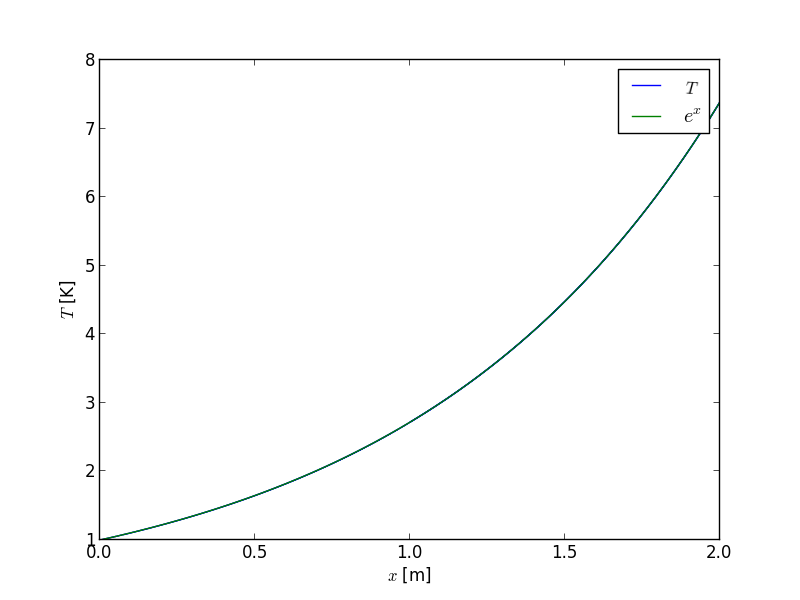
\includegraphics[width=\columnwidth]{plots/output.png}
\caption{Manufactured Solution}
\label{fig:output}
\end{figure}

The method of manufactured solutions forces the solution to a known
equation, which allows error to be quantified.
\subsection*{Derivation}
\begin{equation}\label{eq:heatequ}\frac{dkdT}{dx^2} + q + S = 0\end{equation}
Starting with the heat equation \eqref{eq:heatequ}, we plug in the desired solution \eqref{eq:ex} to T. Ideally, a solution should have infinitely many
derivatives so that it is not possible for a truncated Taylor Series to precisely represent the solution. Thus, $T=x$ or $T=1$ would be a poor
choice.
\begin{equation}\label{eq:ex}T = e^x\end{equation}
\begin{equation}\label{eq:heatequmansol}\frac{dkde^x}{dx^2} + q + S = 0\end{equation}
The equation \eqref{eq:heatequmansol} is then solved for the source term
\begin{equation}\label{eq:heatequsource}S = -q - ke^x\end{equation}
The source term \eqref{eq:heatequsource} is then plugged into the solver to force the solution to that value.
\subsection*{Error Quantification}
Once a solution is obtained, error
can be quantified with equation \eqref{eq:exacterror}. Since the solver's solution is discrete, $\epsilon$ can instead be expressed as equation \eqref{eq:approxerror}.
$\epsilon (h)$ can be graphed and the slope compared against $O(h)$ and $O(h^2)$ convergence.
\begin{equation}\label{eq:exacterror}\epsilon = \sqrt{\int_\Omega (\hat T-\tilde T )^2d\Omega}\end{equation}
\begin{equation}\label{eq:approxerror}\epsilon \propto \sqrt{\frac{1}{N}\sum\limits_{i=1}^N (\hat T (x_i)-\tilde T_i)^2}\end{equation}

\section*{Truncation Error}
By evaluating $\epsilon$ with several grid spacings, relationship \eqref{eq:epsilongrid} can be experimentally determined.
\begin{equation}\label{eq:epsilongrid}\epsilon\propto h^n \end{equation}
In fig. \ref{fig:eperror}, it is evident that the error is proportional to $h^2$. Thus, the solver can be confirmed to be second order.
In the region dominated by truncation error, the graph is a straight line. However, the region where round-off error dominates is
identifiable by a lack of smoothness as it is random.
\begin{figure}
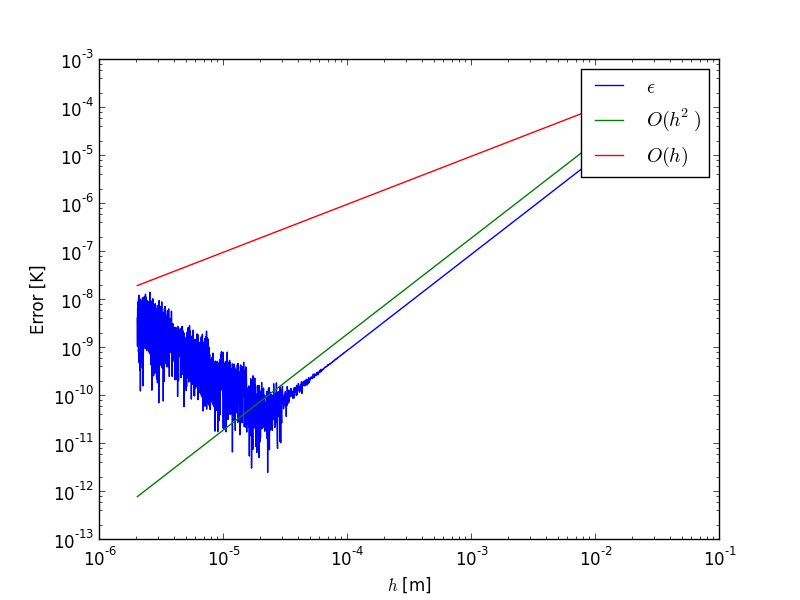
\includegraphics[width=\columnwidth]{plots/eperror.png}
\caption{Extended Precision Solver Error}
\label{fig:eperror}
\end{figure}

\section*{Round-off Error}
Plugging in various values of the significand width into eq. \eqref{eq:fpprecision}. It can be seen that a larger floating point format can represent 
many more significant digits. In general, a trade-off must be made between resource usage and solver accuracy. As floating point precision goes up, the decrease in
solver speed becomes more noticeable as hardware does not natively support the larger formats: Generation of fig. \ref{fig:eperror} took 2 minutes whereas the generation of fig. \ref{fig:qperror} took 2 hours.
It is notable that an increase in grid resolution eventually \emph{must} be followed by an increase in floating point precision.

\begin{figure}\begin{center}\begin{tabularx}{\columnwidth}{|X|X|X|}
\hline
Floating Point Format & Significand Width (bits) & Significant Decimal Digits \\\hline
Single & 24 & 7\\\hline
Double & 53 & 16\\\hline
Extended & 64 & 19\\\hline
Quad & 113 & 34\\\hline
\end{tabularx}\end{center}\label{fg:fpprecision}
\caption{Floating Point Decimal Precision}
\end{figure}

\begin{figure}
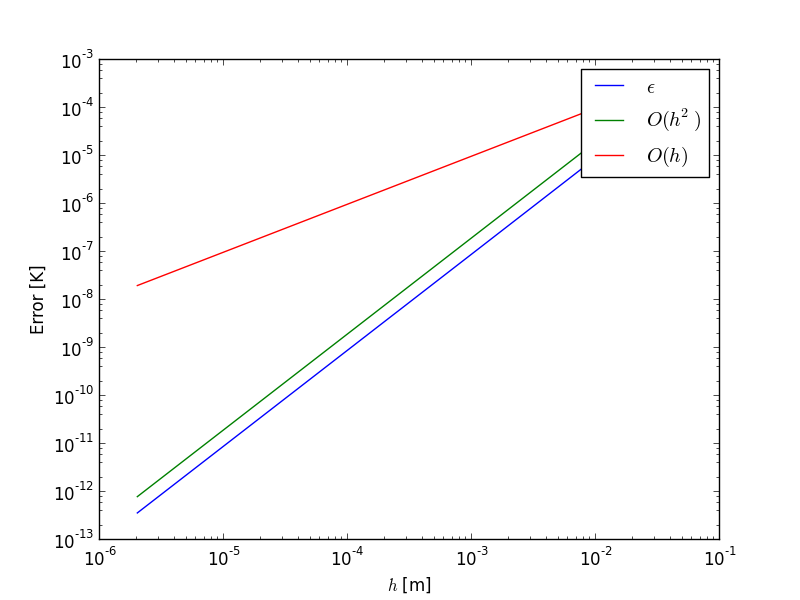
\includegraphics[width=\columnwidth]{plots/qperror.png}
\caption{Quad Precision Solver Error}
\label{fig:qperror}
\end{figure}

\end{document}
